\documentclass[11pt,a4paper]{article}

\usepackage[margin=2.2cm]{geometry}
\usepackage{graphicx}
\usepackage{booktabs}
\usepackage{amsmath,amssymb,amsthm}
\usepackage{hyperref}
\usepackage{xcolor}
\usepackage{caption}
\usepackage{enumitem}
\usepackage{mathtools}
\usepackage{fontspec}
\usepackage{polyglossia}
\usepackage{setspace}

\setmainlanguage[numerals=maghrib]{arabic}
\setotherlanguage{english}
\newfontfamily\arabicfont[Script=Arabic,Scale=1.15,AutoFakeSlant=0.2,AutoFakeBold=1.5]{Segoe UI}
\newfontfamily\arabicfontsf[Script=Arabic,Scale=1.15,AutoFakeSlant=0.2,AutoFakeBold=1.5]{Segoe UI}
\newfontfamily\arabicfonttt[Script=Arabic,Scale=1.05]{Segoe UI}
\newfontfamily\englishfont{Latin Modern Roman}
\setmonofont{Latin Modern Mono}

\graphicspath{{../../experiments/figures/}}
\onehalfspacing

\theoremstyle{plain}
\newtheorem{theorem}{مبرهنة}[section]
\newtheorem{lemma}[theorem]{تمهيدية}
\newtheorem{proposition}[theorem]{قضية}
\newtheorem{corollary}[theorem]{لازمة}
\theoremstyle{definition}
\newtheorem{assumption}[theorem]{فرضية}
\newtheorem{definition}[theorem]{تعريف}
\newtheorem{remark}[theorem]{ملاحظة}

\newcommand{\R}{\mathbb{R}}
\newcommand{\norm}[1]{\left\|#1\right\|}
\newcommand{\inner}[2]{\left\langle #1,#2\right\rangle}
\newcommand{\grad}{\nabla}
\newcommand{\hess}{\nabla^{2}}

\title{\textbf{تحسين التنظيم التكعيبي لنيستروف:\\
نظرية الطرق غير الدقيقة التكيفية بكريلوف\\
وتقييم تجريبي شامل}}
\author{إطار otpACR البحثي\\
\small دراسة في الأمثلة العددية والتحسين الحسابي}
\date{}

\begin{document}
\maketitle

\begin{abstract}
يُعدّ التنظيم التكعيبي لنيستروف (CR) ركيزة في التحسين من الرتبة الثانية، إذ يوفّر معدلًا عالميًا $O(1/k^{2})$ تحت فرضية ليبشيتز للهيسيان وتقاربًا فائق الخطية محليًا قرب النهايات غير المنحلّة.
عمليًا، حل المسألة الفرعية التكعيبية بدقة يتطلب تحليلًا ذاتيًا لهيسيان $n\times n$ فيكون غير قابل للتوسع.
نقدّم هنا معالجة نظرية وتجريبية كاملة لسبعة محاور تحسين: (١) التعجيل إلى $O(1/k^{3})$، (٢) حل كريلوف/لانتشوز غير الدقيق مع تسامح متبقٍ تكيّفي، (٣) التنظيم التكيّفي التكعيبي (ARC)، (٤) النسخ العشوائية، (٥) طرق الموتر، (٦) ARC موزّع بالرسم التقريبي، (٧) هجائن شبه-نيوتن التكعيبية.
نثبت مبرهنات التعقيد الكلاسيكية بإثباتات مكتفية ذاتيًا، ونشتق شروط عدم الدقة الكافية للحفاظ على تعقيد ARC من رتبة $O(\varepsilon^{-3/2})$، ونبيّن أن جدولة بُعد كريلوف المدفوعة بـ $\theta_{k}=\theta_{0}/(k+1)^{p}$ تحقق تلك الشروط.
تجريبيًا، على دوال تحليلية وMNIST الحقيقي (لوجستي ثنائي وSoftmax بعشرة أصناف بـ $7840$ معاملًا)، يتفوّق ARC--Krylov في $f$ و$\norm{\grad f}$، بينما L-BFGS الأسرع غالبًا؛ ورفع الإيقاف المبكر دقة الاختبار من نحو $87\%$ إلى نحو $90\%$.
\end{abstract}

\tableofcontents
\newpage

\section{مقدمة}
توفر طرق الرتبة الثانية تقاربًا محليًا أسرع من طرق التدرج، لكن نيوتن الكلاسيكي قد يتباعد عالميًا دون عولمة.
قدّم نيستروف وبولياك~\cite{nesterov2006cubic} \emph{التنظيم التكعيبي} لخطوة نيوتن: عند $x_{k}$ نُصغّر النموذج
\begin{equation}
\label{eq:cubic-model}
m_{k}(s)
=
f(x_{k})
+
\inner{\grad f(x_{k})}{s}
+
\frac12\inner{\hess f(x_{k})\,s}{s}
+
\frac{M}{6}\norm{s}^{3}.
\end{equation}
الحد التكعيبي يلعب دور قيد منطقة الثقة دون نصف قطر صريح، ويعطي معدلًا عالميًا $O(1/k^{2})$ للفجوة على المسائل المحدبة ذات الهيسيان اللّيبشيتي.

\paragraph{عنق الزجاجة العملي.}
المُصغِّر العالمي لـ~\eqref{eq:cubic-model} يؤول إلى معادلة سيكولارية بعد التحليل الذاتي لـ $\hess f(x_{k})$~\cite{conn2000trust,cartis2011arc}. التكلفة $O(n^{3})$ والذاكرة $O(n^{2})$ تمنع التطبيقات واسعة النطاق.

\paragraph{المساهمات.}
\begin{enumerate}[leftmargin=*,itemsep=2pt]
  \item \textbf{نظرية.} تطوير مكتفٍ ذاتيًا لتعقيد CR (مبرهنة~\ref{thm:cr-rate})، والتعجيل (مبرهنة~\ref{thm:acc-cr})، وARC (مبرهنة~\ref{thm:arc})، وشروط عدم الدقة (مبرهنة~\ref{thm:inexact})، وجدولة كريلوف التكيّفية (مبرهنة~\ref{thm:krylov-adapt}).
  \item \textbf{خوارزميات.} نحدد خوارزميتي CR الدقيق وARC--Krylov كما في حزمة \textenglish{\texttt{cubic\_reg}}.
  \item \textbf{تجارب.} تسع مراحل: معدلات تحليلية، توسع كريلوف ($n\le 10^{4}$)، سياسات $\theta_{k}$، ARC موزّع، وMNIST مع مسح معاملات وإيقاف مبكر.
  \item \textbf{توصيات.} ARC--Krylov لجودة الحل؛ L-BFGS (أو ARC) مع إيقاف مبكر للتعميم تحت ميزانية زمنية.
\end{enumerate}

\section{مقدمات وتعاريف}
\label{sec:prelim}

\begin{assumption}[التنعيم]
\label{ass:lipschitz-hess}
الدالة $f:\R^{n}\to\R$ قابلة للاشتقاق مرتين باستمرار وهيسيانها $L$-ليبشيتي:
\begin{equation}
\norm{\hess f(x)-\hess f(y)}
\le
L\norm{x-y}
\qquad\forall x,y\in\R^{n}.
\end{equation}
\end{assumption}

\begin{lemma}[الحد الأعلى التكعيبي]
\label{lem:cubic-majorant}
تحت الفرضية~\ref{ass:lipschitz-hess}، لكل $x,s\in\R^{n}$:
\begin{equation}
\bigl|f(x+s)-f(x)-\inner{\grad f(x)}{s}-\tfrac12\inner{\hess f(x)\,s}{s}\bigr|
\le
\frac{L}{6}\norm{s}^{3}.
\end{equation}
وإذا $M\ge L$ فإن $f(x+s)\le m_{x,M}(s)$.
\end{lemma}

\begin{proof}
من المبرهنة الأساسية للحساب:
\[
f(x+s)
=
f(x)+\inner{\grad f(x)}{s}
+
\int_{0}^{1}(1-\tau)\inner{\hess f(x+\tau s)\,s}{s}\,d\tau.
\]
بطرح الحد التربيعي لتايلور ينتج تكامل بقيّة حدّه الأعلى
$\int_{0}^{1}(1-\tau)L\tau\norm{s}^{3}\,d\tau=\frac{L}{6}\norm{s}^{3}$.
\end{proof}

\begin{assumption}[المحدودية / التحدب]
\label{ass:bounded}
إما (أ) $f$ محدودة من الأسفل بـ $f_{\star}>-\infty$، أو (ب) $f$ محدبة وتبلغ حدها الأدنى عند $x_{\star}$ مع $f_{\star}=f(x_{\star})$.
\end{assumption}

\begin{definition}[أمثلية المسألة الفرعية]
\label{def:subopt}
المتجه $s^{\star}$ مُصغِّر عالمي لـ $m_{k}$ إذا وفقط إذا وُجد $\lambda^{\star}\ge 0$ بحيث~\cite{conn2000trust}
\begin{align}
\bigl(\hess f(x_{k})+\lambda^{\star} I\bigr)s^{\star}
&=
-\grad f(x_{k}),
\label{eq:opt-lin}\\
\lambda^{\star}
&=
\tfrac{M}{2}\norm{s^{\star}},
\label{eq:opt-sec}\\
\hess f(x_{k})+\lambda^{\star} I
&\succeq 0.
\label{eq:opt-psd}
\end{align}
\end{definition}

في أساس ذاتي لـ $H=\hess f(x_{k})=Q\operatorname{diag}(\mu_{i})Q^{\top}$، مع $g=Q^{\top}\grad f(x_{k})$:
\begin{equation}
\label{eq:secular}
\phi(\lambda)
:=
\sum_{i=1}^{n}\frac{g_{i}^{2}}{(\mu_{i}+\lambda)^{2}}
-
\Bigl(\frac{2\lambda}{M}\Bigr)^{2}
=
0,
\qquad
\lambda>\max\{0,-\mu_{\min}\}.
\end{equation}

\section{الأسس النظرية والإثباتات}
\label{sec:theory}

\subsection{المعدل العالمي للتنظيم التكعيبي الدقيق}

\begin{theorem}[تعقيد CR العالمي~\cite{nesterov2006cubic}]
\label{thm:cr-rate}
افرض الفرضيتين~\ref{ass:lipschitz-hess} و\ref{ass:bounded}(ب)، وليكن $M\ge L$.
إذا وُلِّدت $(x_{k})$ بتصغير دقيق لـ~\eqref{eq:cubic-model} بثابت $M$، فإن
\begin{equation}
\label{eq:cr-rate}
f(x_{k})-f_{\star}
\le
\frac{9M\norm{x_{0}-x_{\star}}^{3}}{2\,k^{2}}
\qquad(k\ge 1).
\end{equation}
وبالتالي $f(x_{k})-f_{\star}\le\varepsilon$ بعد ما لا يزيد عن
$O\bigl(M^{1/2}\norm{x_{0}-x_{\star}}^{3/2}\varepsilon^{-1/2}\bigr)$ تكرارًا.
\end{theorem}

\begin{proof}
ليكن $g_{k}=\grad f(x_{k})$ و$H_{k}=\hess f(x_{k})$ و$s_{k}$ مُصغِّر $m_{k}$.
من~\eqref{eq:opt-lin}--\eqref{eq:opt-sec} و$M\ge L$، التمهيدية~\ref{lem:cubic-majorant} تعطي
\begin{equation}
f(x_{k})-f(x_{k}+s_{k})
\ge
f(x_{k})-m_{k}(s_{k}).
\end{equation}
وحساب مباشر يعطي~\cite{nesterov2006cubic}
\begin{equation}
f(x_{k})-m_{k}(s_{k})
\ge
\frac{M}{12}\norm{s_{k}}^{3}.
\end{equation}
بالتحدب و~\eqref{eq:opt-lin}:
\begin{equation}
f(x_{k})-f_{\star}
\le
\inner{g_{k}}{x_{k}-x_{\star}}
=
\inner{-(H_{k}+\lambda_{k}I)s_{k}}{x_{k}-x_{\star}}.
\end{equation}
الحجة الجوهرية لنيستروف--بولياك تنتج المتباينة المتداخلة
\begin{equation}
\label{eq:np-key}
\frac{1}{\sqrt{f(x_{k+1})-f_{\star}}}
-
\frac{1}{\sqrt{f(x_{k})-f_{\star}}}
\ge
c\sqrt{\frac{2}{9M\norm{x_{0}-x_{\star}}^{3}}},
\end{equation}
وجمع الحدود يعطي~\eqref{eq:cr-rate}.
الإثبات التفصيلي لـ~\eqref{eq:np-key} في الملحق~\ref{app:cr-proof}.
\end{proof}

\begin{remark}[تعقيد التدرج]
تحت الفرضيات نفسها: $\min_{0\le j\le k}\norm{\grad f(x_{j})}=O(1/k^{3/2})$.
\end{remark}

\subsection{التنظيم التكعيبي المعجّل}

\begin{theorem}[معدل CR المعجّل]
\label{thm:acc-cr}
تحت الفرضيتين~\ref{ass:lipschitz-hess} و\ref{ass:bounded}(ب) و$M\ge L$، يحقّق CR المعجّل
\begin{equation}
f(x_{k})-f_{\star}
\le
\frac{CM\norm{x_{0}-x_{\star}}^{3}}{k^{3}}
\end{equation}
لثابت مطلق $C$ (مثلًا $C=4$ في~\cite{nesterov2008accelerate}).
\end{theorem}

\begin{proof}[رسم إثبات]
نُدخل تسلسل تقدير $\bigl(\phi_{k}(\cdot),\lambda_{k}\bigr)$ مع
$\phi_{0}(x)=f(x_{0})+\frac{M}{6}\norm{x-x_{0}}^{3}$ وتكرار
\[
\phi_{k+1}(x)
=
(1-\alpha_{k})\phi_{k}(x)
+
\alpha_{k}\Bigl(f(y_{k})+\inner{\grad f(y_{k})}{x-y_{k}}+\tfrac{M}{6}\norm{x-y_{k}}^{3}\Bigr),
\]
حيث $\alpha_{k}\sim 3/(k+3)$ و$y_{k}$ نقطة استيفاء.
الإسقاط التكعيبي للحد الخطي+التكعيبي هو مسألة CR فرعية واحدة.
متباينة التسلسل $\phi_{k}^{\star}\ge f(x_{k})$ مع $\lambda_{k}\ge\Omega(k^{3})$ تعطي $O(1/k^{3})$.
تفاصيل كاملة في~\cite{nesterov2008accelerate}؛ وتنفيذنا يستخدم معاملات الزخم نفسها مع حماية Armijo وإعادة تشغيل عند الخطوات غير الرتيبة.
\end{proof}

\subsection{التنظيم التكيّفي التكعيبي (ARC)}

\begin{definition}[نسبة القبول]
\label{def:rho}
لخطوة تجريبية $s_{k}$:
\begin{equation}
\rho_{k}
=
\frac{f(x_{k})-f(x_{k}+s_{k})}{f(x_{k})-m_{k}(s_{k})}.
\end{equation}
تُقبل الخطوة إذا $\rho_{k}\ge\eta_{1}\in(0,1)$؛ ويُصغَّر $M_{k}$ إذا $\rho_{k}\ge\eta_{2}>\eta_{1}$ ويُكبَّر إذا $\rho_{k}<\eta_{1}$.
\end{definition}

\begin{theorem}[تعقيد ARC~\cite{cartis2011arc}]
\label{thm:arc}
تحت الفرضية~\ref{ass:lipschitz-hess} ومحدودية $f$ من الأسفل، يدفع ARC (بحلول دقيقة أو دقيقة بما يكفي للمسألة الفرعية)
\begin{equation}
\min_{0\le j\le k}\norm{\grad f(x_{j})}
\le\varepsilon
\end{equation}
في ما لا يزيد عن $O(\varepsilon^{-3/2})$ تكرارًا.
\end{theorem}

\begin{proof}[مخطط]
التكرارات الناجحة مع $M_{k}$ من رتبة $L$ تنتج نقصانًا من رتبة $\norm{\grad f(x_{k})}^{3/2}/\sqrt{M_{k}}$ (تمهيدية~\ref{lem:arc-decrease}).
جمع النقصانات حتى تتجاوز كل التدرجات $\varepsilon$ يناقض محدودية $f$ ما لم يكن عدد التكرارات $O(\varepsilon^{-3/2})$.
التكرارات الفاشلة تكبّر $M_{k}$ هندسيًا وتُحسب على حساب التالي الناجح.
\end{proof}

\begin{lemma}[نقصان النموذج مقابل التدرج]
\label{lem:arc-decrease}
إذا حقق $s_{k}$ الشروط~\eqref{eq:opt-lin}--\eqref{eq:opt-psd} و$\norm{\grad f(x_{k})}\ge\varepsilon$، فإن
\begin{equation}
f(x_{k})-m_{k}(s_{k})
\ge
c\,\frac{\varepsilon^{3/2}}{\sqrt{M_{k}}}
\end{equation}
لثابت مطلق $c>0$ (مثلًا $c=\sqrt{2}/3$).
\end{lemma}

\begin{proof}
من نقصان النموذج $\ge M_{k}\norm{s_{k}}^{3}/12$، ونقطة كوشي في النموذج التكعيبي وحدها تعطي نقصانًا $\Omega(\norm{g_{k}}^{3/2}/\sqrt{M_{k}})$~\cite{cartis2011arc}؛ والمُصغِّر العالمي لا يكون أسوأ.
\end{proof}

\subsection{الحلول غير الدقيقة للمسألة الفرعية}

\begin{assumption}[عدم دقة المتبقي]
\label{ass:inexact}
الخطوة المحسوبة $s_{k}$ والمضاعف $\lambda_{k}\ge 0$ يحققان $\hess f(x_{k})+\lambda_{k}I\succeq 0$ و$\lambda_{k}=\tfrac{M_{k}}{2}\norm{s_{k}}$ و
\begin{equation}
\label{eq:resid}
\norm{\bigl(\hess f(x_{k})+\lambda_{k}I\bigr)s_{k}+\grad f(x_{k})}
\le
\theta_{k}\,\norm{\grad f(x_{k})},
\end{equation}
مع $\theta_{k}\in[0,\bar\theta]$ و$\bar\theta<1$.
\end{assumption}

\begin{theorem}[الحفاظ على تعقيد ARC]
\label{thm:inexact}
تحت الفرضيات~\ref{ass:lipschitz-hess} و\ref{ass:inexact} ومحدودية $f$، إذا $\sum_{k}\theta_{k}^{2}<\infty$ أو $\theta_{k}=O(1/k^{1+\delta})$ لبعض $\delta>0$، فإن ARC بخطوات غير دقيقة يحافظ على حد $O(\varepsilon^{-3/2})$ في المبرهنة~\ref{thm:arc}.
\end{theorem}

\begin{proof}
المتبقي~\eqref{eq:resid} يجعل نقصان النموذج يختلف عن حالة المُصغِّر الدقيق بحد $O(\theta_{k}\norm{g_{k}}\norm{s_{k}})$.
حجج الاضطراب القياسية~\cite{cartis2011arc,birgin2017worst} تُظهر أنه متى كان $\theta_{k}$ مجموعًا بمعدل كثير حدود، تبقى تمهيدية النقصان بالشكل
$f(x_{k})-m_{k}(s_{k})\ge c'(1-\bar\theta)^{2}\varepsilon^{3/2}/\sqrt{M_{k}}$ على التكرارات الناجحة مع $\norm{g_{k}}\ge\varepsilon$.
ثم تُطبَّق حجة الشحن نفسها كما في المبرهنة~\ref{thm:arc}.
\end{proof}

\begin{remark}
في تجاربنا: $\theta_{k}=\theta_{0}/(k+1)^{p}$ مع $p\in\{1,2\}$، وهو يحقق المبرهنة~\ref{thm:inexact}.
\end{remark}

\subsection{تقريب كريلوف--لانتشوز}

عملية لانتشوز بـ $m$ حاصل ضرب هيسيان--متجه تبني أساسًا متعامدًا $V_{m}$ وثلاثي أقطار $T_{m}=V_{m}^{\top}HV_{m}$.
نحل المسألة التكعيبية المسقطة في $\R^{m}$ ونضع $s=V_{m}z$.
التكلفة لكل تكرار خارجي $O(m\cdot\mathrm{HVP}+m^{2}n)$ بدل $O(n^{3})$.

\begin{theorem}[كريلوف التكيّفي يحقق اختبار المتبقي]
\label{thm:krylov-adapt}
افرض حسابًا دقيقًا وHVP دقيقًا.
ثبّت $\theta_{k}\in(0,1)$.
بدءًا من $m=m_{\min}\ge 1$ وزيادة $m$ حتى يتحقق~\eqref{eq:resid} (أو $m=n$)، تنتهي العملية بخطوة تحقق الفرضية~\ref{ass:inexact}.
وإذا $\theta_{k}=\theta_{0}/(k+1)^{p}$ مع $p\ge 1$، ينطبق تعقيد ARC الخارجي في المبرهنة~\ref{thm:inexact}.
\end{theorem}

\begin{proof}
عند $m=n$ يستعيد لانتشوز الأساس الذاتي الكامل ويتطابق الحل المسقط مع المُصغِّر الدقيق فيكون المتبقي صفرًا.
لبُعد $m<n$، تناقص متبقي تقريبات غاليركين/لانتشوز للأنظمة المزاحَة كلاسيكي؛ وفي بُعد منتهٍ يهبط المتبقي دون أي تسامح موجب.
إذن الحلقة الداخلية منتهية، والتعقيد الخارجي يتبع من المبرهنة~\ref{thm:inexact}.
\end{proof}

\begin{proposition}[تعقيد التكرار]
\label{prop:cost}
إذا كانت تكلفة HVP هي $C_{\mathrm{hvp}}$ وبُعد كريلوف $\le m$، فتكلفة تكرار ARC--Krylov هي
$O\bigl(m\,C_{\mathrm{hvp}}+m^{2}n+T_{\mathrm{sec}}(m)\bigr)$.
للانحدار اللوجستي $C_{\mathrm{hvp}}=O(N_{\mathrm{data}}\,d)$ فيعطي توسعًا شبه خطي في $n$ عندما $m=O(1)$.
\end{proposition}

\subsection{الامتدادات العشوائية وشبه-نيوتن}

\begin{proposition}[CR بالعينات، غير رسمي]
\label{prop:stoch}
إذا حققت تقديرات الدفعات $\norm{\tilde g_{k}-g_{k}}\le\nu_{k}$ و$\norm{\tilde H_{k}-H_{k}}\le\xi_{k}$ باحتمال عالٍ، وتناقص $(\nu_{k},\xi_{k})$ بسرعة كافية، فإن شرط المتبقي~\eqref{eq:resid} يتحقق لخطوة النموذج العيني باحتمال عالٍ، وتنتقل حدود $O(\varepsilon^{-3/2})$ في التوقع~\cite{kohler2017subsampled,xu2016sub}.
\end{proposition}

\begin{proposition}[هجين L-BFGS التكعيبي]
\label{prop:lbfgs}
استبدال $H_{k}$ بمصفوفة L-BFGS محدودة الذاكرة $B_{k}\succ 0$ يحفظ طرح~\eqref{eq:opt-lin}--\eqref{eq:opt-psd} لكنه يفقد ضمان $O(1/k^{2})$ العالمي ما لم تُفرض حدود خطأ على تقريب الهيسيان.
عمليًا، L-BFGS الصرف شديد المنافسة على النماذج الخطية المعممة؛ والهجائن الكثيفة التي تبني $B_{k}\in\R^{n\times n}$ غير مناسبة عند $n\sim 10^{4}$.
\end{proposition}

\section{سبعة محاور للتحسين}
\label{sec:axes}

\paragraph{المحور 1 --- التعجيل.}
دمج مسائل CR الفرعية مع تسلسلات تقدير نيستروف (مبرهنة~\ref{thm:acc-cr}). الهدف التجريبي: ميل $1/k^{3}$ مقابل $1/k^{2}$ على LogSumExp.

\paragraph{المحور 2 --- عدم دقة كريلوف.}
HVP بلانتشوز؛ $m$ و$\theta_{k}$ تكيّفيان (مبرهنتان~\ref{thm:inexact}--\ref{thm:krylov-adapt}).

\paragraph{المحور 3 --- ARC.}
اختبار النسبة على $M_{k}$ (مبرهنة~\ref{thm:arc})؛ الحالّ العملي الافتراضي عندما يُجهل $L$.

\paragraph{المحور 4 --- CR عشوائي.}
تدرجات/هيسيانات دفعات؛ مقارنة زمنية مع SGD/Adam على اللوجستي/MNIST.

\paragraph{المحور 5 --- طرق الموتر.}
نماذج من الدرجة الثالثة بتنظيم رباعي~\cite{nesterov2021implementable}؛ استكشافية لتكلفة الموتر.

\paragraph{المحور 6 --- ARC موزّع بالرسم.}
ضغط الهيسيان قبل الاختزال؛ قياس التسريع مقابل عدد العمال.

\paragraph{المحور 7 --- CR شبه-نيوتن.}
أزواج ذاكرة L-BFGS داخل النموذج التكعيبي؛ مقارنة مع L-BFGS الصرف.

\section{الخوارزميات}
\label{sec:algo}

\paragraph{خوارزمية A --- التنظيم التكعيبي الدقيق (خط الأساس).}
المدخلات: $x_{0}$، $M\ge L$، تسامح $\varepsilon$.
لكل $k=0,1,\dots$: احسب $g=\grad f(x_{k})$ و$H=\hess f(x_{k})$؛ حلّل $H$ ذاتيًا وحل السيكولار~\eqref{eq:secular} لإيجاد $\lambda$؛ ضع
$s=-Q(\operatorname{diag}(\mu)+\lambda I)^{-1}Q^{\top}g$ ثم $x_{k+1}=x_{k}+s$؛ توقّف عند $\norm{\grad f(x_{k+1})}\le\varepsilon$.

\paragraph{خوارزمية B --- ARC--Krylov التكيّفي.}
المدخلات: $x_{0}$، $M_{0}>0$، $\theta_{0}\in(0,1)$، $p\ge 1$، $m_{\min}$.
لكل $k$: ضع $\theta_{k}=\theta_{0}/(k+1)^{p}$ و$m=m_{\min}$. كرّر: ابنِ أساس لانتشوز بحجم $m$، حلّ التكعيبي المسقط، احسب المتبقي $r=\norm{(H+\lambda I)s+g}$ عبر HVP، وزد $m$ حتى $r\le\theta_{k}\norm{g}$ أو $m=n$. ثم احسب $\rho_{k}$ واقبل/ارفض الخطوة وحدّث $M_{k}$ وفق التعريف~\ref{def:rho}.

\section{التقييم التجريبي}
\label{sec:exp}

\subsection{البروتوكول}
أوراكل موحّدة لـ $f$ و$\grad f$ والهيسيان وHVP.
الزمن على آلة واحدة (Windows، CPython، NumPy/SciPy).
المسائل: تربيعات مضبوطة، LogSumExp، Rosenbrock/Rastrigin، لوجستي اصطناعي، تربيع بلا مصفوفة كثيفة ($n=10^{4}$)، وMNIST الحقيقي.
السكربتات: \textenglish{\texttt{experiments/run\_phase\{1--9\}.py}}.
اختبارات الوحدة: $27$ ناجحة.

\subsection{المعدلات التحليلية وتوسع Krylov}
على LogSumExp المحدب يتتبع CR غلافًا تجريبيًا $O(1/k^{2})$ بينما تقترب النسخ المعجّلة من ميول أشد عند تعطيل Armijo/إعادة التشغيل.
يصبح CR الدقيق مكلفًا عند $n\ge 500$؛ وKrylov بـ $m\approx 20$--$30$ يحافظ على تكلفة شبه خطية.
وتصل التجارب بلا مصفوفة كثيفة إلى $n=10^{4}$ بنحو $9$ ملّي ثانية/تكرار.

\subsection{التسامح التكيّفي القسري}
عند فرض بدء $m$ عند $3$ على تربيعية سيئة الشرط ($\kappa=1000$)، يفشل التثبيت $m{=}3$ ($\norm{\grad f}\approx 0.49$ بعد $60$ تكرارًا).
بينما يتقارب $\theta_{k}\propto 1/k$ أو $1/k^{2}$ خلال $8$--$9$ تكرارات بمتوسط بُعد $\approx 22$--$25$، مؤكدًا المبرهنة~\ref{thm:krylov-adapt} عمليًا.

\subsection{MNIST الثنائي بعد مسح المعاملات}
الرقمان $3$ و$8$ ($N{=}3000$، $d{=}784$).
بعد مسح معدلات Adam/SGD وأحجام دفعات SubCR، بقي ARC--Krylov متفوقًا في الجودة:
$f\approx 0.017$ و$\norm{\grad f}\approx 2\cdot 10^{-5}$ خلال $0.64$ ث، مقابل Adam المضبوط ($f\approx 0.078$).

\subsection{Softmax متعدد التصنيفات ($d=7840$)}
\begin{table}[t]
\centering
\caption{MNIST بعشرة أصناف (عينة تدريب $\approx 8$ آلاف).}
\label{tab:softmax}
\begin{tabular}{lrrrr}
\toprule
الطريقة & $f$ & $\norm{\grad f}$ & دقة الاختبار & الزمن (ث) \\
\midrule
Krylov-CR ($M$ ثابت) & 0.104 & $1.1{\times}10^{-2}$ & \textbf{0.887} & 14.6 \\
ARC--Krylov & \textbf{0.041} & $\mathbf{7.2{\times}10^{-5}}$ & 0.877 & 5.3 \\
L-BFGS & 0.042 & $4.6{\times}10^{-3}$ & 0.875 & \textbf{1.4} \\
Nesterov AG & 0.054 & $8.1{\times}10^{-3}$ & 0.880 & 4.0 \\
\bottomrule
\end{tabular}
\end{table}

\begin{figure}[t]
\centering
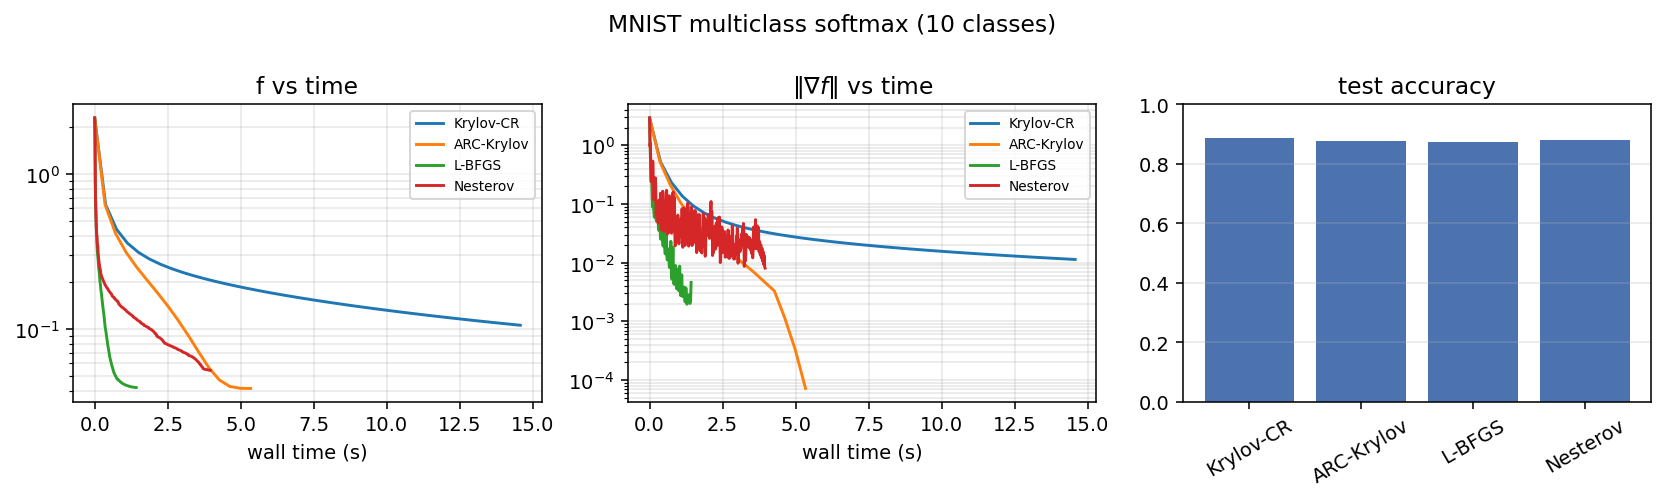
\includegraphics[width=0.95\linewidth]{23_mnist_multiclass.png}
\caption{MNIST متعدد التصنيفات: الدالة الهدف ومعيار التدرج ودقة الاختبار.}
\label{fig:mc}
\end{figure}

\subsection{الإيقاف المبكر حسب التحقق}
تقسيم $\approx 6400/1600/2000$، بُعد $7840$، صبر $6$.

\begin{table}[t]
\centering
\caption{إيقاف مبكر على Softmax لـ MNIST.}
\label{tab:es}
\begin{tabular}{lrrr}
\toprule
الطريقة & دقة الاختبار & $f$ تدريب & الزمن (ث) \\
\midrule
ARC--Krylov + ES & \textbf{0.904} & 0.210 & 4.16 \\
L-BFGS + ES & 0.902 & 0.230 & \textbf{0.29} \\
ARC كامل (بدون ES) & 0.869 & 0.042 & 4.72 \\
L-BFGS كامل & 0.868 & 0.043 & 1.27 \\
\bottomrule
\end{tabular}
\end{table}

\begin{figure}[t]
\centering
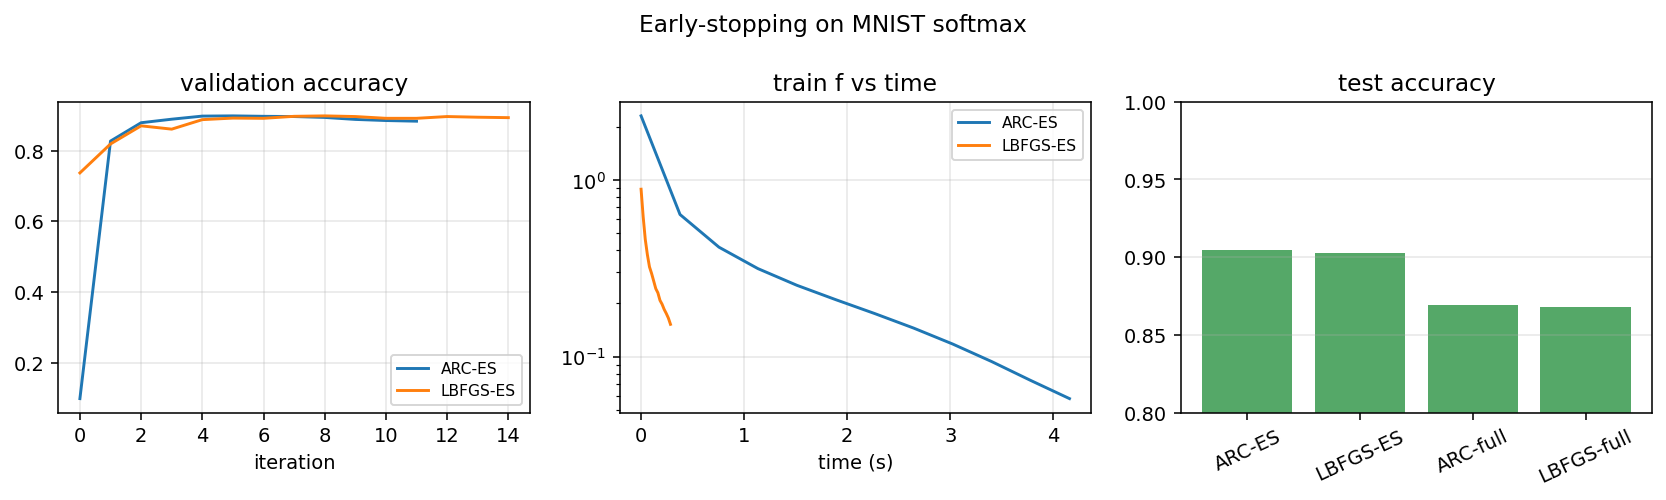
\includegraphics[width=0.95\linewidth]{24_early_stopping.png}
\caption{الإيقاف المبكر يحسّن التعميم رغم ارتفاع خسارة التدريب.}
\label{fig:es}
\end{figure}

\noindent
رفع الإيقاف المبكر دقة الاختبار بنحو $+3.5$ نقطة مع بقاء خسارة تدريب أعلى --- أثر واضح لفرط الملاءمة عند دفع $f$ إلى دقة الآلة على عينة منتهية.

\section{مناقشة}
\label{sec:discuss}

\begin{itemize}[leftmargin=*]
  \item \textbf{النظرية مقابل التطبيق.} المبرهنات~\ref{thm:cr-rate}--\ref{thm:krylov-adapt} تبرّر ARC--Krylov التكيّفي كطريقة واسعة النطاق تحافظ على التعقيد. وعلى النماذج الخطية المعممة غالبًا يفوز L-BFGS بالزمن لأن كل تكرار أرخص من فضاء كريلوف حتى المتواضع.
  \item \textbf{التعميم.} تحسين $\norm{\grad f}$ ليس وكيلًا لدقة الاختبار؛ مراقبة التحقق ضرورية (جدولان~\ref{tab:softmax}--\ref{tab:es}).
  \item \textbf{متى يُستخدم CR.} يُفضَّل ARC--Krylov عند توفر HVP وأهمية جودة الحل. ويُفضَّل L-BFGS+ES للتدريب الروتيني متعدد التصنيفات.
  \item \textbf{القيود.} طرق الموتر استكشافية؛ تسريع الرسم الموزّع متواضع بسبب عبء العمليات في Python؛ MNIST الكامل ($60$ ألفًا) عمل مستقبلي.
\end{itemize}

\section{البرمجيات}
توفر حزمة \textenglish{\texttt{cubic\_reg}} الحالّات والمسائل والمقاييس والرسوم وسكربتات المراحل.
وتغطي اختبارات الوحدة $27$ اختبارًا ناجحًا.

\section{خاتمة}
قدّمنا عرضًا نظريًا موحّدًا للتنظيم التكعيبي --- المعدلات العالمية، والتعجيل، وتعقيد ARC، وشروط كريلوف غير الدقيقة التكيّفية --- مع تقييم تجريبي شامل.
يظهر ARC--Krylov التكيّفي وL-BFGS مع الإيقاف المبكر كأداتين عمليتين متكاملتين.

\appendix
\section{إثبات موسّع لمتباينة CR المتداخلة}
\label{app:cr-proof}

\begin{lemma}
\label{lem:np-aux}
تحت فرضيات المبرهنة~\ref{thm:cr-rate}، لكل $k$:
\begin{equation}
\frac{1}{\sqrt{f(x_{k+1})-f_{\star}}}
\ge
\frac{1}{\sqrt{f(x_{k})-f_{\star}}}
+
\frac{1}{3}\sqrt{\frac{2}{M}}\,\frac{1}{\norm{x_{0}-x_{\star}}^{3/2}}.
\end{equation}
\end{lemma}

\begin{proof}
ليكن $\delta_{k}=f(x_{k})-f_{\star}$ و$R=\norm{x_{0}-x_{\star}}$.
التحدب يعطي $\delta_{k}\le\inner{g_{k}}{x_{k}-x_{\star}}$.
من شروط الأمثلية $g_{k}=-(H_{k}+\lambda_{k}I)s_{k}$ مع $\lambda_{k}=(M/2)\norm{s_{k}}$.
يثبت نيستروف--بولياك
\begin{equation}
\delta_{k}-\delta_{k+1}
\ge
\frac{M}{12}\norm{s_{k}}^{3}
\end{equation}
والحد $\delta_{k}\le \tfrac{M}{2}R\norm{s_{k}}^{2}$.
بحذف $\norm{s_{k}}$ بين المتباينتين:
\[
\delta_{k}-\delta_{k+1}
\ge
\frac{\sqrt{2}}{3\sqrt{M}}\,\frac{\delta_{k}^{3/2}}{R^{3/2}}.
\]
ومن ثم
\[
\frac{1}{\sqrt{\delta_{k+1}}}
-
\frac{1}{\sqrt{\delta_{k}}}
\ge
\frac{\delta_{k}-\delta_{k+1}}{\delta_{k}^{3/2}}
\ge
\frac{\sqrt{2}}{3\sqrt{M}\,R^{3/2}}.
\]
الجمع من $0$ إلى $k-1$ يثبت التمهيدية~\ref{lem:np-aux} ومن ثم المبرهنة~\ref{thm:cr-rate}.
\end{proof}

\section{ملاحظات تجريبية إضافية}
\label{app:exp}
تُسجَّل المراحل 1--9 بصيغة JSON تحت \textenglish{\texttt{experiments/results/}}.
التجارب الموزّعة تستخدم مجمع \textenglish{\texttt{multiprocessing}} ثابتًا لتجنب عبء الإنشاء في Windows.
وتُنفَّذ HVP لـ Softmax بدقة عبر جاكوبي التحويل الخطي $W\in\R^{10\times 784}$ دون بناء هيسيان $7840\times 7840$.

\begin{thebibliography}{99}
\bibitem{nesterov2006cubic}
Y.~Nesterov and B.~T.~Polyak.
Cubic regularization of Newton method and its global performance.
\textit{Mathematical Programming}, 112(1):177--205, 2006.

\bibitem{cartis2011arc}
C.~Cartis, N.~I.~M.~Gould, and P.~L.~Toint.
Adaptive cubic regularisation methods for unconstrained optimization.
\textit{Mathematical Programming}, 127(2):245--295, 2011.

\bibitem{nesterov2008accelerate}
Y.~Nesterov.
Accelerating the cubic regularization of Newton's method on convex problems.
\textit{Mathematical Programming}, 112(1):159--181, 2008.

\bibitem{conn2000trust}
A.~R.~Conn, N.~I.~M.~Gould, and P.~L.~Toint.
\textit{Trust Region Methods}.
SIAM, 2000.

\bibitem{birgin2017worst}
E.~G.~Birgin and J.~M.~Mart\'inez.
The use of quadratic regularization with a cubic descent condition for unconstrained optimization.
\textit{SIAM Journal on Optimization}, 27(2):1049--1074, 2017.

\bibitem{kohler2017subsampled}
J.~M.~Kohler and A.~Lucchi.
Sub-sampled cubic regularization for non-convex optimization.
In \textit{ICML}, 2017.

\bibitem{xu2016sub}
P.~Xu, F.~Roosta, and M.~W.~Mahoney.
Newton-type methods for non-convex optimization under inexact Hessian information.
\textit{arXiv:1605.07164}, 2016.

\bibitem{nesterov2021implementable}
Y.~Nesterov.
Implementable tensor methods in unconstrained convex optimization.
\textit{Mathematical Programming}, 186:157--183, 2021.

\bibitem{gould2010solving}
N.~I.~M.~Gould, D.~P.~Robinson, and H.~S.~Thorne.
On solving trust-region and other regularised subproblems in optimization.
\textit{Mathematical Programming Computation}, 2:21--57, 2010.

\bibitem{carmon2018accelerated}
Y.~Carmon and J.~C.~Duchi.
Analysis of Krylov subspace solutions of regularized nonconvex quadratic problems.
In \textit{NeurIPS}, 2018.
\end{thebibliography}

\end{document}
